% chapter 1
\chapter{Introduction}
\label{chap:01_introduction}

\section{Architecture}
\label{sec:architecture}
The DLX processor serves as a \textbf{32-bit RISC architecture} that closely resembles the MIPS model. It operates on a \textbf{5-stage in-order pipeline} for integer processing, comprising stages for fetch, decode, execute, memory, and write back. Memory interactions occur via specific \textbf{load} and \textbf{store} commands, and they function in \textbf{big-endian mode}. \\

Initially, in the \textbf{fetch stage}, an instruction is retrieved from the \textit{Instruction Memory}. After a single clock cycle, the instruction moves to the \textbf{decode stage} and here the addresses of the involved registers are identified and sent to the \textit{Register File}, which subsequently reads and outputs the corresponding values. Simultaneously, if an immediate value is present, it is extracted and sign-extended for use in later stages. During the \textbf{execution stage}, the \textit{Arithmetic Logic Unit (ALU)} receives the appropriate input values, which may either come directly from the previous stage or be forwarded from one of the two subsequent stages, courtesy of the \textit{Forwarding Unit}. Concurrently, a specialized module evaluates whether the first of the two registers value is zero, particularly relevant for branch operations. In the \textbf{memory stage}, the \textit{DRAM} is accessed as needed, and jump conditions are assessed. Finally, during the \textbf{write back stage}, output values are channeled through designated \textit{multiplexers}. \\

The subsequent chapters will provide a detailed explanation of each of these stages, as well as the methodologies employed to mitigate hazards and ensure reliable operation of the processor. %A schematic representation of the DLX processor is presented in Figure~\ref{fig:dlx_architecture}.

%\begin{figure}[!htbp]
%    \centering
%    \includegraphics[width=0.6\textwidth]{source/figures/dlx_architecture.png}
%    \caption{Schematic diagram of DLX architecture}
%    \label{fig:dlx_architecture}
%\end{figure}

\section{Instruction Set}
\label{sec:instruction_set}
Instructions in this architecture have a uniform 32-bit length and they can be classified into three principal categories:
\begin{itemize}%[nosep]
    \item \texttt{I-Type} operations;
    \item \texttt{R-Type} operations;
    \item \texttt{J-Type} operations.
\end{itemize}

Irrespective of the instruction class, a 6-bit opcode field is invariably included. The opcode's nature dictates how the remaining 26 bits are interpreted, as illustrated in Figure~\ref{fig:instruction_format}. \\

\begin{figure}[!htbp]
    \centering
    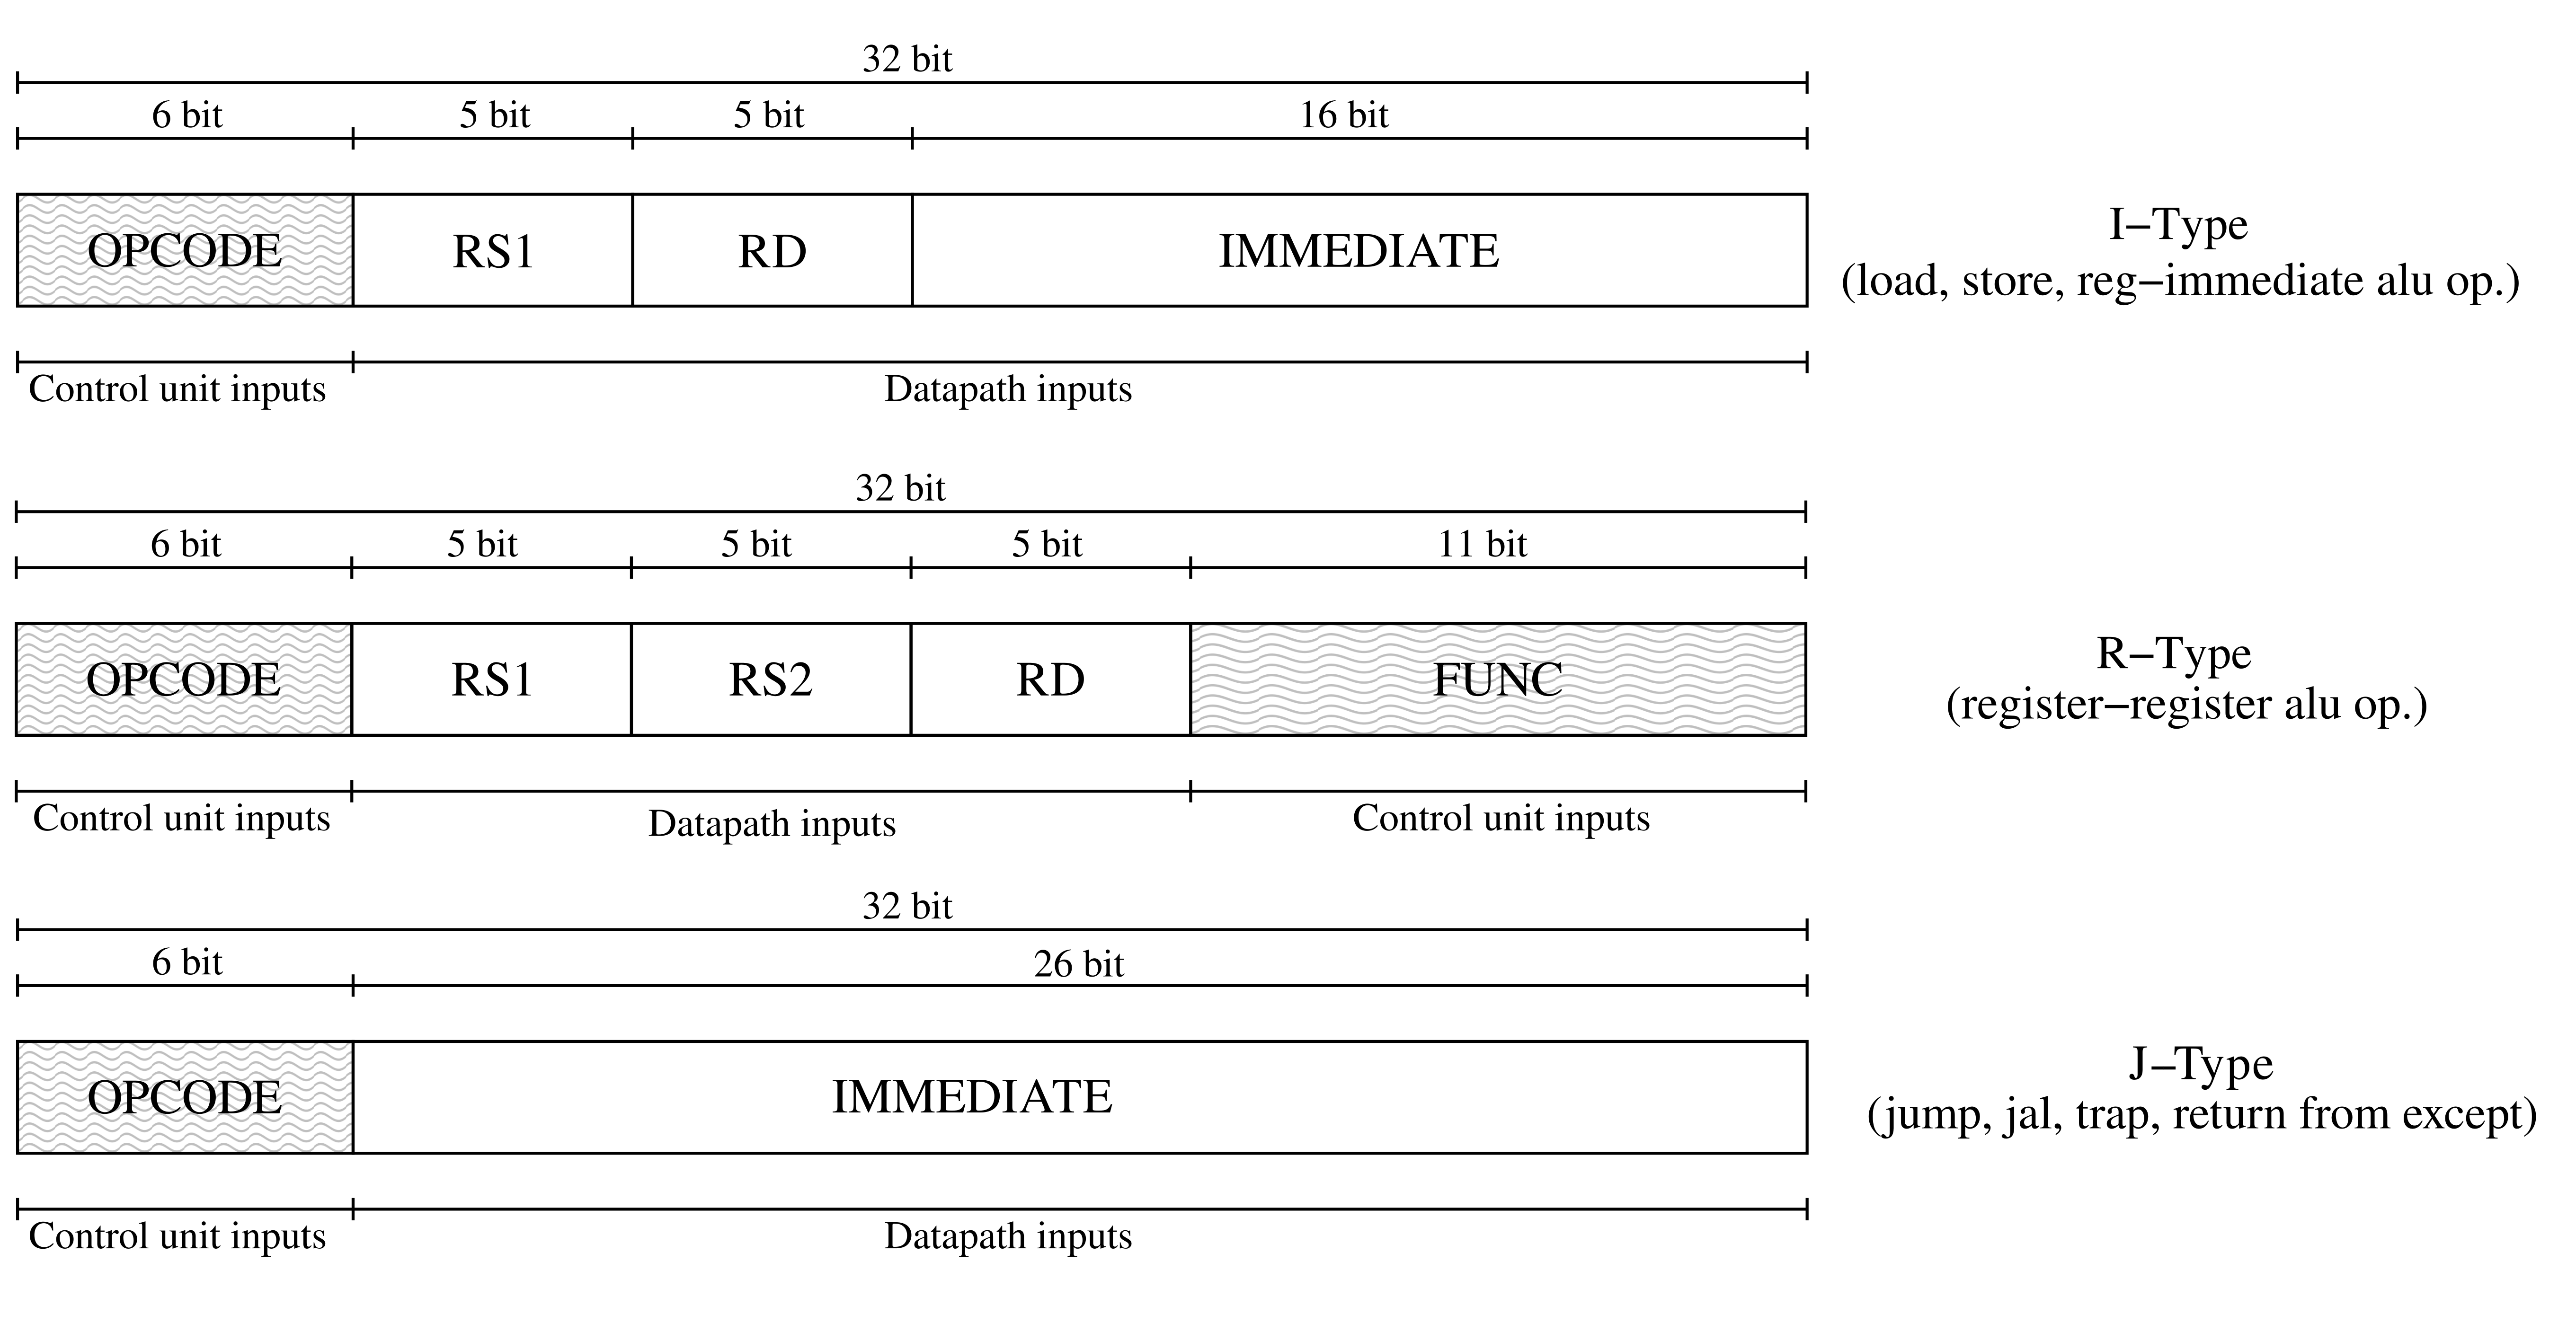
\includegraphics[width=0.9\textwidth]{source/figures/instruction_formats.png}
    \caption{Instruction Formats}
    \label{fig:instruction_format}
\end{figure}

The processor is designed to implement a specific subset of the DLX ISA, comprising the following categories. Instructions shown as \underline{underlined} are exclusive to the pro version of the processor.

\subsection{Arithmetic Operations}
These instructions perform basic arithmetic operations such as addition, subtraction and multiplication. The computed result is stored in a designated destination register. The operands for these operations can either be two source registers or a source register and an immediate numerical value as the second operand.

\begin{itemize}%[nosep]
	\item \texttt{ADD}: an R-Type operation for adding the values in source registers.
	\item \underline{\texttt{ADDU}}: an R-Type operation for the addition of unsigned integers from source registers.
	\item \texttt{ADDI}: an I-Type operation that adds an immediate value to a source register.
	\item \underline{\texttt{ADDUI}}: an I-Type operation for adding an unsigned immediate value to a source register.
	\item \texttt{SUB}: an R-Type operation for subtracting the values of source registers.
	\item \underline{\texttt{SUBU}}: an R-Type operation for the subtraction of unsigned integers from source registers.
	\item \texttt{SUBI}: an I-Type operation for subtracting an immediate value from a source register.
	\item \underline{\texttt{SUBUI}}: an I-Type operation for subtracting an unsigned immediate value from a source register.
	\item \underline{\texttt{MULT}}: an R-Type operation for multiplying the values of source registers.
	\item \underline{\texttt{MULTU}}: an R-Type operation for multiplying unsigned values of a source register.
\end{itemize}

\subsection{Shift Operations}
These commands allow the shifting of binary digits within a register, either to the left or to the right. The right shifts can be either logical or arithmetic in nature.

\begin{itemize}%[nosep]
	\item \texttt{SLL}: an R-Type operation that performs a logical left shift on the source register by the number of positions specified in another source register.
	\item \texttt{SLLI}: an I-Type operation that performs a logical left shift on the source register by the number of positions specified by the immediate value.
	\item \texttt{SRL}: an R-Type operation that executes a logical right shift on the source register by a count specified in another source register.
	\item \texttt{SRLI}: an I-Type operation that carries out a logical right shift on the source register by the number of positions dictated by the immediate value.
	\item \underline{\texttt{SRA}}: an R-Type operation that conducts an arithmetic right shift on the source register by the number of positions indicated in another source register.
	\item \underline{\texttt{SRAI}}: an I-Type operation that performs an arithmetic right shift on the source register by the number of positions given by the immediate value.
\end{itemize}

\subsection{Logical Operations}
These instructions help in bitwise manipulation and logical comparisons between source registers or between a source register and an immediate value.

\begin{itemize}%[nosep]
	\item \texttt{AND}: an R-Type operation that performs a bitwise AND between the source registers.
	\item \texttt{ANDI}: an I-Type operation that executes a bitwise AND between a source register and an immediate value.
	\item \texttt{XOR}: an R-Type operation that performs a bitwise XOR between the source registers.
	\item \texttt{XORI}: an I-Type operation that carries out a bitwise XOR between a source register and an immediate value.
	\item \texttt{OR}: an R-Type operation that executes a bitwise OR between the source registers.
	\item \texttt{ORI}: an I-Type operation that performs a bitwise OR between a source register and an immediate value.
\end{itemize}

\subsection{Comparison Operations}
These instructions compare the values in source registers or a source register and an immediate value and write 1 to the destination register if the condition is satisfied.

\begin{itemize}%[nosep]
	\item \underline{\texttt{SEQ}}: an R-Type instruction comparing two source registers to determine if they are equal.
	\item \underline{\texttt{SEQI}}: an I-Type instruction comparing a source register with an immediate value to determine if they are equal.
 
	\item \texttt{SNE}: an R-Type instruction comparing two source registers to determine if they are not equal.
	\item \texttt{SNEI}: an I-Type instruction comparing a source register with an immediate value to determine if they are not equal.

	\item \texttt{SGE}: an R-Type instruction comparing two source registers to ascertain if the first is greater than or equal to the second.
	\item \texttt{SGEU}: an R-Type instruction for unsigned comparison between two source registers to determine if the first is greater than or equal to the second.
	\item \texttt{SGEI}: an I-Type instruction comparing a source register and an immediate value to check if the first is greater than or equal to the second.
	\item \texttt{SGEUI}: an I-Type instruction for unsigned comparison between a source register and an immediate value, checking if the first is greater than or equal to the second.
 
	\item \underline{\texttt{SLT}}: an R-Type instruction comparing two source registers to ascertain if the first is less than the second.
	\item \underline{\texttt{SLTU}}: an R-Type instruction for unsigned comparison between two source registers to determine if the first is less than the second.
	\item \underline{\texttt{SLTI}}: an I-Type instruction comparing a source register and an immediate value to check if the first is less than the second.
	\item \underline{\texttt{SLTUI}}: an I-Type instruction for unsigned comparison between a source register and an immediate value, checking if the first is less than the second.
 
 	\item \underline{\texttt{SGT}}: an R-Type instruction comparing two source registers to ascertain if the first is greater than the second.
	\item \underline{\texttt{SGTU}}: an R-Type instruction for unsigned comparison between two source registers to determine if the first is greater than the second.
	\item \underline{\texttt{SGTI}}: an I-Type instruction comparing a source register and an immediate value to check if the first is greater than the second.
	\item \underline{\texttt{SGTUI}}: an I-Type instruction for unsigned comparison between a source register and an immediate value, checking if the first is greater than the second.
 
        \item \underline{\texttt{SLE}}: an R-Type instruction comparing two source registers to ascertain if the first is less than or equal the second.
        \item \underline{\texttt{SLEU}}: an R-Type instruction for unsigned comparison between two source registers to determine if the first is less than or equal the second.
	\item \underline{\texttt{SLEI}}: an I-Type instruction comparing a source register and an immediate value to check if the first is less than or equal the second.
	\item \underline{\texttt{SLEUI}}: an I-Type instruction for unsigned comparison between a source register and an immediate value, checking if the first is less than or equal the second.
\end{itemize}

\subsection{Jumps and Branches}
These instructions handle conditional and unconditional branching. They redirect the program's execution flow to a specific instruction address, either by offsetting the current Program Counter (PC) or by setting it to an absolute address. Some of these instructions also save the return address in a designated register, specifically \texttt{R31}.

\begin{itemize}%[nosep]
	\item \texttt{J}: a J-Type instruction that performs a relative jump to a target instruction, specified by adding an immediate value to the PC (Program Counter).
	\item \texttt{JAL}: a J-Type instruction that conducts a relative jump as specified by adding the PC and an immediate value. Additionally, stores the pre-jump PC incremented by 4 into the destination register.
	\item \underline{\texttt{JR}}: a I-Type instruction that executes an absolute jump to the instruction address specified by the immediate value.
	\item \underline{\texttt{JALR}}: a I-Type instruction that carries out an absolute jump to an instruction address specified by the immediate value. Before jumping, it also saves the current PC value incremented by 4 into the destination register.
	\item \texttt{BEQZ}: An I-Type instruction employed for conditional branching when the value in the specified register is equal to zero.
	\item \texttt{BNEZ}: An I-Type instruction employed for conditional branching when the value in the specified register is not equal to zero.
\end{itemize}

\subsection{Load and Store Instructions}
These instructions manage the transfer of data between the register file and the memory. The load instruction reads data from a specific memory address within the DRAM and stores it into a designated register in the Register File. Meanwhile, the store instruction writes data from the Register File to a specified memory location within the DRAM. In both cases, the target memory address is often calculated using an immediate value.

\begin{itemize}%[nosep]
	\item \texttt{LW}: an I-Type instruction for reading a 32-byte signed value from the data memory.
	%\item \texttt{LHU}: an I-Type instruction for reading a 16-byte unsigned value from data memory.
	%\item \texttt{LB}: an I-Type instruction for reading an 8-byte signed value from the data memory.
	%\item \texttt{LBU}: an I-Type instruction for reading an 8-byte unsigned value from data memory.
	\item \texttt{SW}: an I-Type instruction to store a 32-bit value from an integer source register into the data memory.
	%\item \texttt{SB}: an I-Type instruction for storing an 8-bit value from an integer source register into the data memory.
	%\item \texttt{SF}: an I-Type instruction that stores a 32-bit value from a floating-point source register into the data memory.
\end{itemize}

\subsection{General-purpose Operations}
These instructions perform a general-purpose operations that may not fit cleanly into other categories.

\begin{itemize}%[nosep]
	\item \texttt{NOP}: an I-Type instruction that performs no operation.
	\item \underline{\texttt{LHI}}: an I-Type instruction that loads a 16-bit immediate value into the most significant half of the integer register.
	%\item \texttt{MOVFP}: an R-Type instruction that transfers the value from an integer register to another integer register.
\end{itemize}

\paragraph{Notes}

Programmers must be vigilant as the processor supports a branch delay slot. This means inserting three NOP instruction after each branching and jumping command to preclude unintended outcomes.

% Basic Functions
%\begin{itemize}[nosep]
%	\item add
%	\item addi
%	\item and
%	\item andi
%	\item beqz
%	\item bnez
%	\item j
%	\item jal
%	\item lw
%	\item nop
%	\item or
%	\item ori
%	\item sge
%	\item sgei
%	\item sle
%	\item slei
%	\item sll
%	\item slli
%	\item sne
%	\item snei
%	\item srl
%	\item srli
%	\item sub
%	\item subi
%	\item sw
%	\item xor
%	\item xori
%\end{itemize}

\section{Software}
\label{sec:software}
This section offers a concise overview of the software tools deployed for the simulation, synthesis and physical implementation of the DLX architecture within the context of this project.

\subsection{Questa Sim}
Used for simulation, Questa Sim-64 version 2020.4 for Linux x86\_64 is the core simulation and debug engine of the Questa verification solution by Siemens. Questa Sim also natively supports multiple key technologies such as SystemVerilog for Testbench, UPF, UCIS, and OVM/UVM, setting it apart from ModelSim in terms of performance, capacity, and features.

\subsection{Design Compiler}
For synthesis, we utilized Design Compiler Graphical, version S-2021.06-SP4 for Linux64 systems and developed by Synopsys. This tool can be accessed via a UNIX shell using either the \texttt{dc\_shell}/\texttt{dc\_shell-xg} commands or the \texttt{dc\_shell-t}/\texttt{dc1\_shell-xg-t} commands. The former set of commands utilizes a Synopsys-specific proprietary language, while the latter employs the more standardized Tcl language. The focus of this project is solely on the Tcl-based version of the Design Compiler.

\subsection{Innovus Implementation System}
The physical implementation for this project was carried out using the Cadence Innovus Implementation System, version v20.11-s130\_1. Innovus is specifically designed to cater to the requirements of contemporary system-on-chip (SoC) developers. It offers cutting-edge advancements in power, performance, and area (PPA) metrics, while simultaneously accelerating time-to-market. Furthermore, Innovus incorporates machine learning-driven capabilities and is part of the Cadence Safety Solution.
